Studiamo adesso in dettaglio il legame chimico tramite la teoria degli orbitali molecolari.

Ciò significa che studieremo il legame nelle molecole, sebbene sappiamo che ci sono molti sistemi che non esistono sotto forma molecolare, ossia ci sono composti fortemente ionici dei quali conosciamo i solidi ma non le molecole. Ne è un esempio l'NaCl: la specie molecolare del cloruro di sodio non esiste, ma esiste il solido.

Dobbiamo allora comprendere perché non esistano le molecole singole delle speci fortementi ioniche, per poi ragionare sul legame chimico, che ha una natura diversa nei sistemi molecolari.

Dobbiamo quindi rispondere a una serie di domande:
\begin{itemize}
    \item Perché si formano le molecole, dato che molti sistemi non esistono come tali?
    \item Quali condizioni bisogna soddisfare affinché il composto che si forma a seguito di una reazione, sia stabile?
    \item Perché esistono geometrie ben definite?
\end{itemize}
Prima di andare avanti va da ricordare che in linea generale se facciamo reagire una specie A con una specie B otterremo una specie C in modo spontaneo solo se l'energia del sistema diminuisce. 

Ricordiamo poi che qualunque stato legato avrà un'energia potenziale negativa: in un sistema AB dove A e B sono due atomi, essi sono legati se la loro energia potenziale è minore di zero. Se per qualche motivo l'energia dovesse aumentare, nell'istante in cui essa diventasse pari a zero gli atomi non sarebbero più legati.

Ragioniamo solo sull'energia potenziale per via dell'esistenza del teorema del viriale, il quale afferma che "\textit{La variazione dell'energia totale di un sistema ha lo stesso segno della variazione dell'energia potenziale}". Quindi la molecola AB si formerà nel momento in cui l'energia potenziale dei due atomi A e B diminuisce (fino a diventare negativa) man mano che li avviciniamo.\\

La toeria degli orbitali molecolari è applicabile solo nel caso di molecole semplici. Nel momento in cui volessimo studiare sistemi più complessi, bisogna usare una catalogazione precedente, che si basava sul tipo di legame presente tra le molecole in esame.
Un parametro estremamente utile a comprendere i sistemi è il concetto di elettronegatività, che è la tendenza che hanno i diversi atomi ad attrarre su di sé la carica di legame. Nel momento in cui uno dei due atomi costituenti il nucleo è abbastanza più elettronegativo dell'altro, si avrà una dislocazione della carica di legame, per cui diremo che la molecola avrà una sua polarità, ossia avrà struttura simile a quella di un dipolo perché avrà una parziale carica positiva e una parziale carica negativa.

In base al valore della differenza di elettronegatività, il legame verrà etichettato in vari modi:
\begin{itemize}
    \item Se è piccola (fino a 0.4) si parla di \textbf{legame covalente};
    \item Se inizia a crescere ma è comunque contenuta (da 0.4 fino a 1.9) si parla di \textbf{legame} covalente \textbf{polare}, e la molecola avrà una polarità cospicua. 
    \item Se diventa molto grande (da 1.9 in poi) si parla di \textbf{legame ionico}.
\end{itemize} 
\subsection{Il legame polare}
In questo caso ci saranno parziali cariche positive e negative, che possono venire indicate in diversi modi: o rispettivamente con $\delta^+$ e $\delta^-$, o con zone rosse e blu che indicano rispettivamente addensamento di elettroni e le zone che si sono positivizzate, o con una freccia con la punta e una croce, dove la punta è rivolta verso l'atomo più elettronegativo.
\subsection{Il legame metallico}
Consideriamo la struttura dei metalli, come ad esempio il sodio:
\begin{figure}[htp]
    \centering
    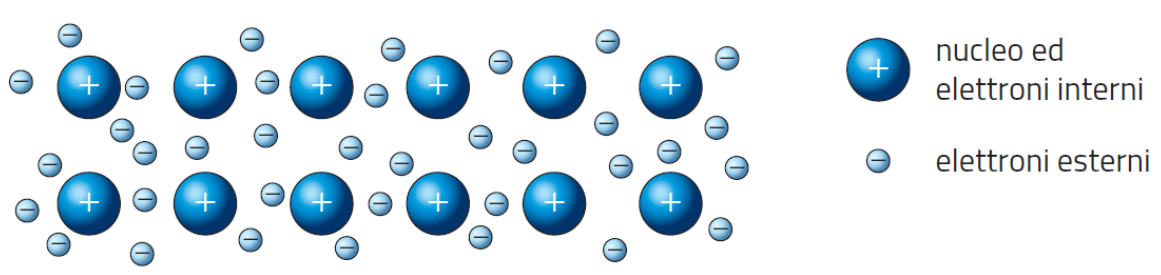
\includegraphics[width=3cm]{immagini/legame-metallico.png}
\end{figure}
Le sferette tutte identiche rappresentano gli atomi, che occupano posizioni ben definite all'interno di una struttura cristallina 
\subsection{Il legame ionico}
in esso la dislocazione delle cariche e totale, per cui immaginiamo che ci sia cessione dell'elettrone e in conseguenza a ciò si formino uno ione positivo e uno negativo.
\subsection{il ciclo di Born-Haber}
\subsection{Esempi vari}
$\bullet$ ES1 \ce{F_2}

\begin{figure}[htp]
    \centering
    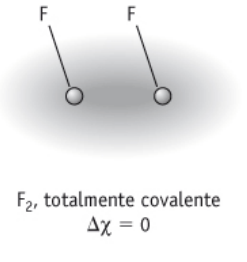
\includegraphics[width=4cm]{immagini/F_2.png}
\end{figure}

$\bullet$ ES2 HF

\begin{figure}[htp]
    \centering
    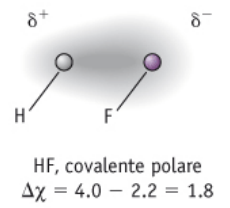
\includegraphics[width=5cm]{immagini/HF.png}
\end{figure}

$\bullet$ ES3 LiF

\begin{figure}[htp]
    \centering
    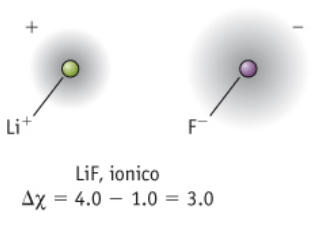
\includegraphics[width=5cm]{immagini/LiF.png}
\end{figure}

$\bullet$ ES4

\begin{figure}[htp]
    \centering
    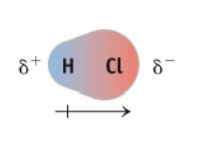
\includegraphics[width=5cm]{immagini/HCl.png}
\end{figure}

$\bullet$ ES5

\begin{figure}[htp]
    \centering
    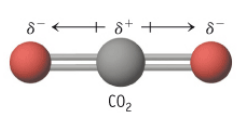
\includegraphics[width=5cm]{immagini/CO_2.png}
\end{figure}

$\bullet$ ES6

\begin{figure}[htp]
    \centering
    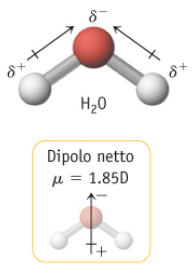
\includegraphics[width=5cm]{immagini/H_2O.png}
\end{figure}

$\bullet$ ES7

\begin{figure}[htp]
    \centering
    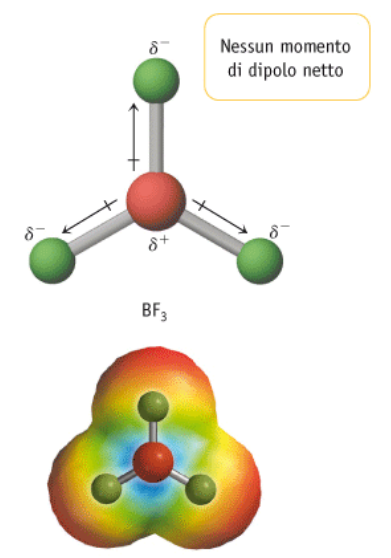
\includegraphics[width=5cm]{immagini/BF_3-dipolo.png}
\end{figure}

$\bullet$ ES8

\begin{figure}[htp]
    \centering
    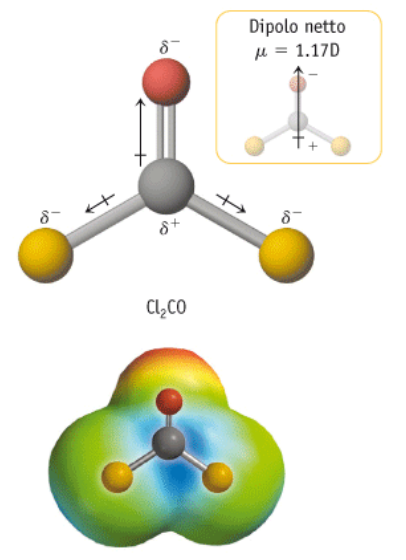
\includegraphics[width=5cm]{immagini/Cl_2CO.png}
\end{figure}

$\bullet$ ES9

\begin{figure}[htp]
    \centering
    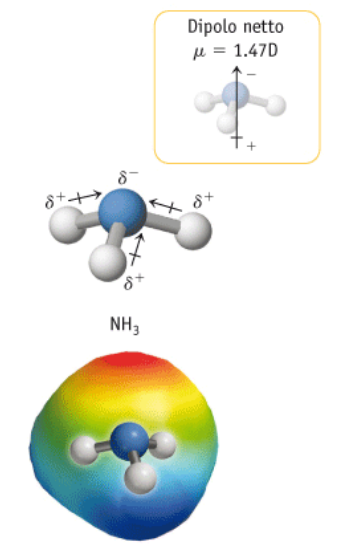
\includegraphics[width=5cm]{immagini/NH_3.png}
\end{figure}

$\bullet$ ES10

\begin{figure}[htp]
    \centering
    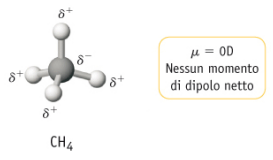
\includegraphics[width=5cm]{immagini/CH_4.png}
\end{figure}

$\bullet$ ES11

\begin{figure}[htp]
    \centering
    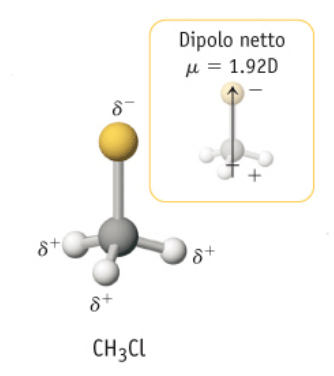
\includegraphics[width=5cm]{immagini/CH_3Cl.png}
\end{figure}

$\bullet$ ES12

\begin{figure}[htp]
    \centering
    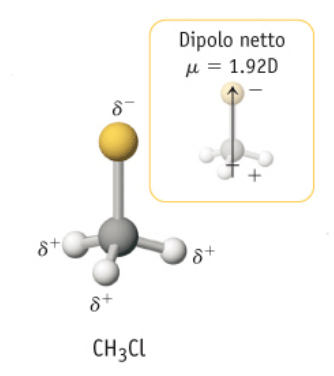
\includegraphics[width=5cm]{immagini/CH_3Cl.png}
\end{figure}

$\bullet$ ES13

\begin{figure}[htp]
    \centering
    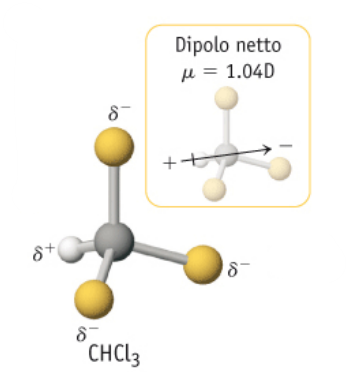
\includegraphics[width=5cm]{immagini/CHCl_3.png}
\end{figure}

$\bullet$ ES14

\begin{figure}[htp]
    \centering
    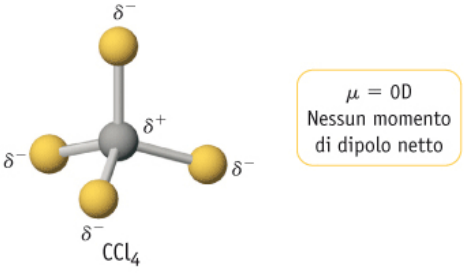
\includegraphics[width=5cm]{immagini/CCl_4.png}
\end{figure}


\subsection{Il legame covalente}